\documentclass{beamer}
\usetheme{metropolis}
\usepackage{graphicx}
\usepackage{subfig}
\usepackage{hyperref}
\usepackage{tcolorbox}
\title{Calculus-Based Physics-1: Mechanics (PHYS150-02): Unit 7}
\date{\today}
\author{Jordan Hanson}
\institute{Whittier College Department of Physics and Astronomy}

\begin{document}
\maketitle

\section{Unit 7 Summary}

\begin{frame}{Unit 7 Summary}
\begin{enumerate}
\item \alert{Work} and \alert{potential energy}
\begin{itemize}
\item \textbf{Lab activity:} Oscillator and gravity trading work and potential energy
\end{itemize}
\item Potential energy and \textbf{conservative forces}
\item \alert{\textbf{Conservation of Energy}}
\begin{itemize}
\item \textit{Calculus review: the fundamental theorem of calculus}
\item Graphical representations of integrals and energy
\end{itemize}
\end{enumerate}
\end{frame}

\section{Work and Potential Energy}

\begin{frame}{Work and potential energy}
When we do work on a system, even if in the final state the system has no velocity, it can still have energy.  The concept of \textit{potential energy} is \textbf{like thinking of work backwards}:
\begin{itemize}
\item If we compress an oscillator (a spring), and keep compressing it, it has no kinetic energy but it will have kinetic energy if we release it.
\item If we raise an object against the force of gravity to a certain height, it has no kinetic energy but it will have kinetic energy if we drop it.
\item \alert{But it took work to create this change in kinetic energy, from the work-energy theorem.} 
\end{itemize}
\textit{Systems are not necessarily \textbf{required} to operate like this...Think of stretching plastic or dough.  Where does the work go?}
\end{frame}

\begin{frame}{Work and potential energy}
The relationship between work and potential energy therefore resembles (by definition) the opposite of the work-energy theorem:
\begin{equation}
\Delta U_{\rm AB} = U_{\rm B} - U_{\rm A} = -W_{\rm AB}
\end{equation}
\end{frame}

\begin{frame}{Work and potential energy}
\begin{figure}
\centering
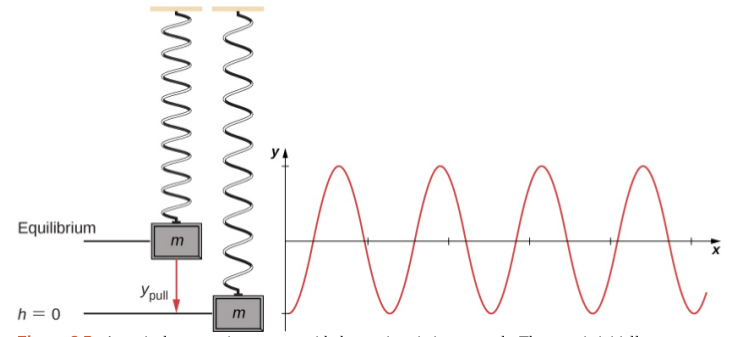
\includegraphics[width=0.9\textwidth,trim=0cm 0.1cm 0cm 0cm,clip=true]{figures/osc.png}
\caption{\label{fig:osc} An oscillator is stretched to a new equilibrium point by gravity.  When pulled a certain distance down, or compressed a certain distance upwards, $y_{\rm pull}$, we observe oscillation.}
\end{figure}
\end{frame}

\begin{frame}{Work and potential energy}
\begin{figure}
\centering
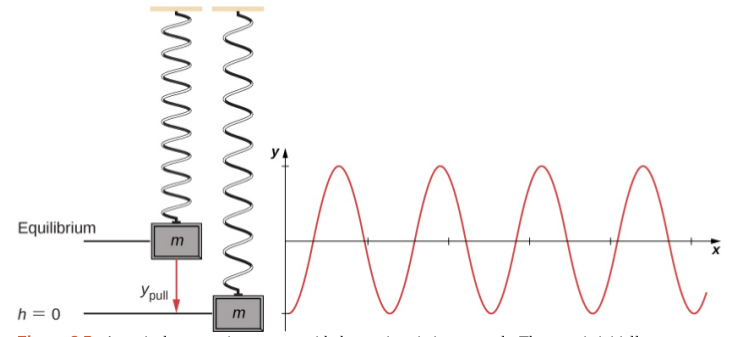
\includegraphics[width=0.9\textwidth,trim=0cm 0.1cm 0cm 0cm,clip=true]{figures/osc.png}
\caption{\label{fig:osc2} Notice that it does not matter what the observer defines as \textit{zero} potential energy, since work is required to perform \textit{changes} in potential energy.}
\end{figure}
\end{frame}

\begin{frame}{Work and potential energy}
\begin{figure}
\centering
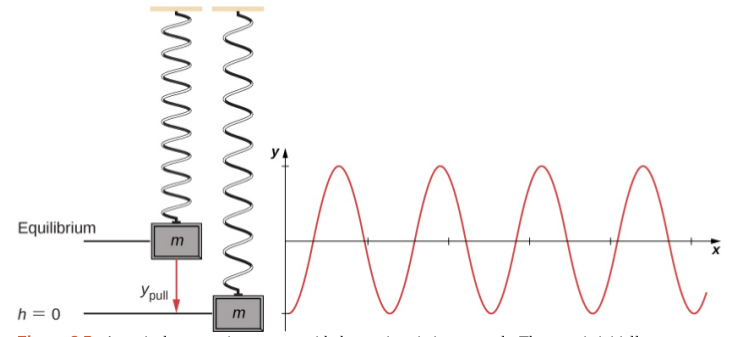
\includegraphics[width=0.9\textwidth,trim=0cm 0.1cm 0cm 0cm,clip=true]{figures/osc.png}
\caption{\label{fig:osc3} The fact that work is required only to perform changes in potential energy, but not does not determine the \textit{absolute scale} of potential energy, means the observer \alert{may choose the location of zero potential energy}, in the same fashion as choosing a coordinate system.}
\end{figure}
\end{frame}

\begin{frame}{Work and potential energy}
\begin{figure}
\centering
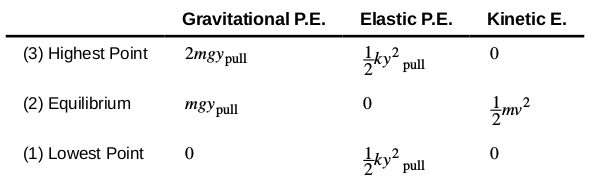
\includegraphics[width=0.9\textwidth,trim=0cm 0.1cm 0cm 0cm,clip=true]{figures/table.png}
\caption{\label{fig:osc4} If a mass $m$ is connected to the oscillator and \textit{we choose} the potential energy zero-point to be \textbf{the low point of oscillation}, the values listed in this table correspond to the energies at various states.}
\end{figure}
\end{frame}

\section{Lab Activity - Gravity and the Oscillator}

\begin{frame}{Lab Activity: Work and Potential Energy}
\small
\begin{itemize}
\item Using the springs, weights, hooks, and system of clamps and grips, build a vertical oscillating system.
\item Diagram the system, showing a clearly defined value for $y_{\rm pull}$, and a clearly defined choice for the potential energy zero-point.
\item Measure the \textit{unstretched} spring length, and the \textit{equilibrium length} caused by gravity, to \textbf{derive the spring constant $k$}.  Quote the value of $k$ in N/m.
\item Pull the spring downwards by $y_{\rm pull}$, and record the maximum and minimum heights of the weight as the spring oscillates it.
\item Create a table like Tab. \ref{fig:osc4}, and fill in the actual energy values in Joules.  What is your predicted value for $v$, the speed at which the weight moves when the oscillator is at the equilibrium position?
\end{itemize}
\end{frame}

\begin{frame}{Work and potential energy}
\begin{figure}
\centering
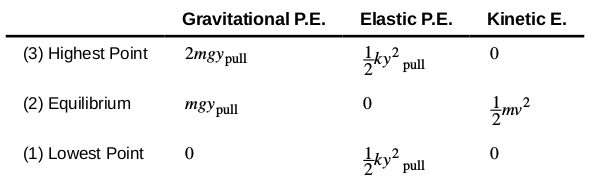
\includegraphics[width=0.9\textwidth,trim=0cm 0.1cm 0cm 0cm,clip=true]{figures/table.png}
\caption{\label{fig:osc5} If a mass $m$ is connected to the oscillator and \textit{we choose} the potential energy zero-point to be \textbf{the low point of oscillation}, the values listed in this table correspond to the energies at various states.}
\end{figure}
\end{frame}

\section{Lab Activity - Gravity and the Oscillator, Part 2}

\begin{frame}{Lab Activity: Work and Potential Energy}
\small
\begin{itemize}
\item Measure the \textit{unstretched} spring length, and the \textit{equilibrium length} caused by gravity, to \textbf{derive the spring constant $k$}.  Quote the value of $k$ in N/m.
\item Pull the spring downwards by $y_{\rm pull}$, and record the maximum and minimum heights of the weight.
\item Create a table like Tab. \ref{fig:osc4}, and fill in the actual energy values in Joules.  What is your predicted value for $v$?
\item Using the \textbf{Vernier LabPro} and the \textit{motion detector attachment}, measure $v$ when the spring is at equilibrium position, and quote the value in m/s.  Does it agree with your prediction based on energy conservation?  Why or why not?
\end{itemize}
\end{frame}

\begin{frame}{Work and potential energy}
\begin{figure}
\centering
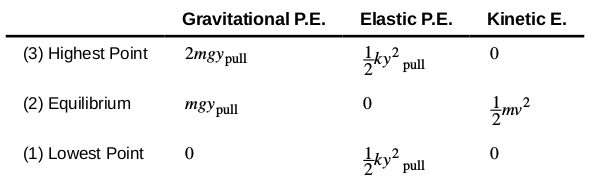
\includegraphics[width=0.9\textwidth,trim=0cm 0.1cm 0cm 0cm,clip=true]{figures/table.png}
\caption{\label{fig:osc6} The value for $v$ is predicted by energy conservation.  What do you measure?}
\end{figure}
\end{frame}

\section{Potential Energy and Conservative Forces}

\begin{frame}{Potential Energy and Conservative Forces}
Let path 1 be be through a force field that does work $W_{\rm 1}$ on a system, and path 2 be a different path that does work $W_{\rm 2}$ on a system.
\begin{equation}
W_{\rm 1} = \int_{\rm Path 1} \vec{F}\cdot d\vec{r} = \int_{\rm Path 2} \vec{F} \cdot d\vec{r} = W_{\rm 2}
\end{equation}
A force is conservative if 
\begin{equation}
W_{\rm 1} = W_{\rm 2}
\end{equation}
Suppose path 1 goes from point A to B, and path 2 returns from B to A.  If the force remains constant, but the path is reversed, then $W_{\rm 1} = -W_{\rm 2}$.  But this means the path is \textit{closed}, so 
\begin{equation}
\oint \vec{F} \cdot d\vec{r} = W_{\rm 1} + W_{\rm 2} = W_{\rm 1} - W_{\rm 1} = 0
\label{eq:work}
\end{equation}
\end{frame}

\section{Conservation of Energy}

\begin{frame}{Conservation of Energy}
Bringing all these concepts together: \alert{\textbf{Conservation of Energy}}. \\ \vspace{1cm}
\begin{tcolorbox}[colback=white,colframe=red!40!blue,title=Conservation of Energy]
\alert{$\Delta (KE + PE) = 0$}
\end{tcolorbox}
\end{frame}

\begin{frame}{Conservation of Energy}
\textit{Recall the notion of a conservative force}.  In your own words, write down the defining characteristics of a conservative force.  Which of these forces is NOT conservative?
\begin{itemize}
\item A: Stoke's Law of viscous drag
\item B: Gravity near Earth's surface
\item C: Hooke's Law
\item D: All are conservative
\end{itemize}
\end{frame}

\begin{frame}{Conservation of Energy}
\begin{figure}
\centering
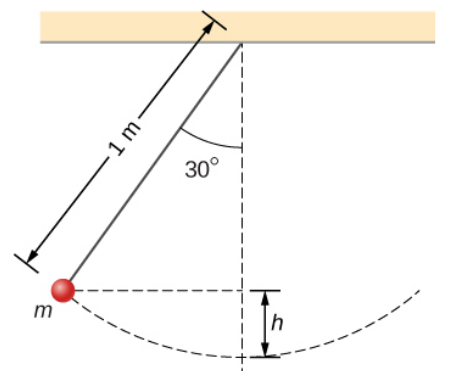
\includegraphics[width=0.5\textwidth]{figures/pend.png}
\end{figure}
\end{frame}

\begin{frame}{Conservation of Energy}
We can show that a \textit{pendulum} exhibits the same properties as a \textit{spring}.  A pendulum is like a spring, where the restoring force is determined by $g$, the gravitational acceleration, and $L$, the length of the pendulum.  That is, $a_{\rm p} = \frac{g}{L}x$, where $x$ is the displacement from equilibrium, and $a$ is the acceleration corresponding to $x$.  (Derivation to follow).  What is the force on a 1 meter-long pendulum suspending a mass of 100 grams if $x=10$ cm?
\begin{itemize}
\item A: 10 N
\item B: 1 N
\item C: 0.1 N
\item D: 0.01 N
\end{itemize}
\end{frame}

\begin{frame}{Conservation of Energy}
The pendulum stores gravitational potential energy $U = mgh$.  Set the zero point of gravitational potential energy to the lowest point of the pendulum.  Show that the potential energy as a function of the angle $\theta$ is \\ \vspace{1cm}
\begin{equation}
U = mgL(1-\cos\theta)
\end{equation}
\end{frame}

\begin{frame}{Conservation of Energy}
At which point in the trajectory of the mass on the end of the pendulum is the velocity the highest?
\begin{itemize}
\item The starting point at the top
\item The lowest point
\item The top point at the side opposite from release point
\item In between the highest and lowest points
\end{itemize}
\end{frame}

\begin{frame}{Conservation of Energy}
By setting pendulum potential energy equal to kinetic energy, show that the maximum velocity achieved by the pendulum mass is
\begin{equation}
v_{\rm max} = \sqrt{2Lg}(1-\cos\theta)^{1/2}
\end{equation}
\end{frame}

\begin{frame}{Conservation of Energy}
If the length of the pendulum is 10 cm, and $g = 10$, and the initial angle is 30 degrees, what is the maximum speed of the pendulum? 
\begin{itemize}
\item 0.1 m/s
\item 0.5 m/s
\item 1 m/s
\item 5 m/s
\end{itemize}
\end{frame}

\begin{frame}{Conservation of Energy}
We can show that the \textit{period} of the pendulum is related to other quantities as follows:
\begin{equation}
T^2 = 4\pi^2 \left(\frac{L}{g}\right)
\end{equation}
Using the PhET simulation below, measure the gravitational acceleration on the moon.  Record your reasoning in lab notebooks. \\ \vspace{1cm}
\url{https://phet.colorado.edu/sims/html/pendulum-lab/latest/pendulum-lab_en.html}
\end{frame}

\begin{frame}{Conservation of Energy}
\small
Conservative forces may be found by taking the negative derivative of the potential energies we've found through the work done: \\ \vspace{0.5cm}
\begin{columns}[T]
\begin{column}{0.5\textwidth}
\centering
\textbf{Potential energy:}
\begin{itemize}
\item $U_{\rm s} = \frac{1}{2}kx^2$
\item $U_{\rm g} = mgy$
\item $U_{\rm p} = mgL(1-\cos\theta)$
\end{itemize}
\end{column}
\begin{column}{0.5\textwidth}
\centering
\textbf{Corresponding force:}
\begin{itemize}
\item $\vec{F} = -kx\hat{i}$
\item $\vec{F} = -mg\hat{j}$
\item $\vec{F} = -\left(\frac{mg}{L}\right)x\hat{i}$
\end{itemize}
\end{column}
\end{columns}
Forces that follow Eq. \ref{eq:work} have to obey
\begin{equation}
\vec{F}(x) = -\frac{dU}{dx}\hat{i}
\end{equation}
We may use conservation of energy to predict the behavior of systems, even when we don't know actual trajectory versus time...
\end{frame}

\begin{frame}{Conservation of Energy}
\small Suppose we encounter a particle with potential energy $U(x) = \frac{1}{2}k x^2 + Ae^{-\frac{1}{2}\left(\frac{x}{\sigma}\right)^2}$.  If the particle has a mass $m$ moving with this potential has a velocity $v_{\rm b}$ when located at $x = b$.  Show that the particle will not cross the origin unless \\ \vspace{0.5cm}
\begin{equation}
A \leq \frac{kb^2 + m v_{\rm b}^2}{2\left(1-e^{-\frac{1}{2}\left(\frac{b}{\sigma}\right)^2}\right)}
\end{equation}
\textbf{Solve in groups at the boards}.  \textit{Hint: Use conservation of energy, assuming the final energy is equal to the potential energy at the origin.}
\end{frame}

\begin{frame}{Conservation of Energy}
\small Notice that if $\frac{1}{2}\left(\frac{b}{\sigma}\right)^2 \ll 1$, then \ \\ \vspace{0.5cm}
\begin{align}
A \lesssim \frac{\frac{1}{2}kb^2 + \frac{1}{2}m v_{\rm b}^2}{\frac{1}{2}\left(\frac{b}{\sigma}\right)^2} &= \frac{E_{\rm i}^0}{\frac{1}{2}\left(\frac{b}{\sigma}\right)^2} \\
\left(\frac{A}{2}\right)\left(\frac{b}{\sigma}\right)^2 \lesssim E_{\rm i}^0
\end{align}
This is odd; why does the initial energy \alert{appear to be \textit{less than} $A$?}  The answer is that, in order to satisfy the limit, $b \ll \sqrt{2}\sigma$.  Thus, the particle has to be close to the origin to cross it, experiencing a gradual wall rather than a sharp one.  \textbf{The corresponding problem in the \textit{quantum limit} leads to quantum tunneling...} 
\end{frame}

\begin{frame}{Conservation of Energy}
\begin{columns}[T]
\begin{column}{0.3\textwidth}
\small
Which particle or particles will cross the origin, if each starts at rest?
\begin{itemize}
\item A: Black only
\item B: Black and Blue
\item C: Blue only
\item D: Red only
\end{itemize}
\end{column}
\begin{column}{0.7\textwidth}
\begin{figure}
\centering
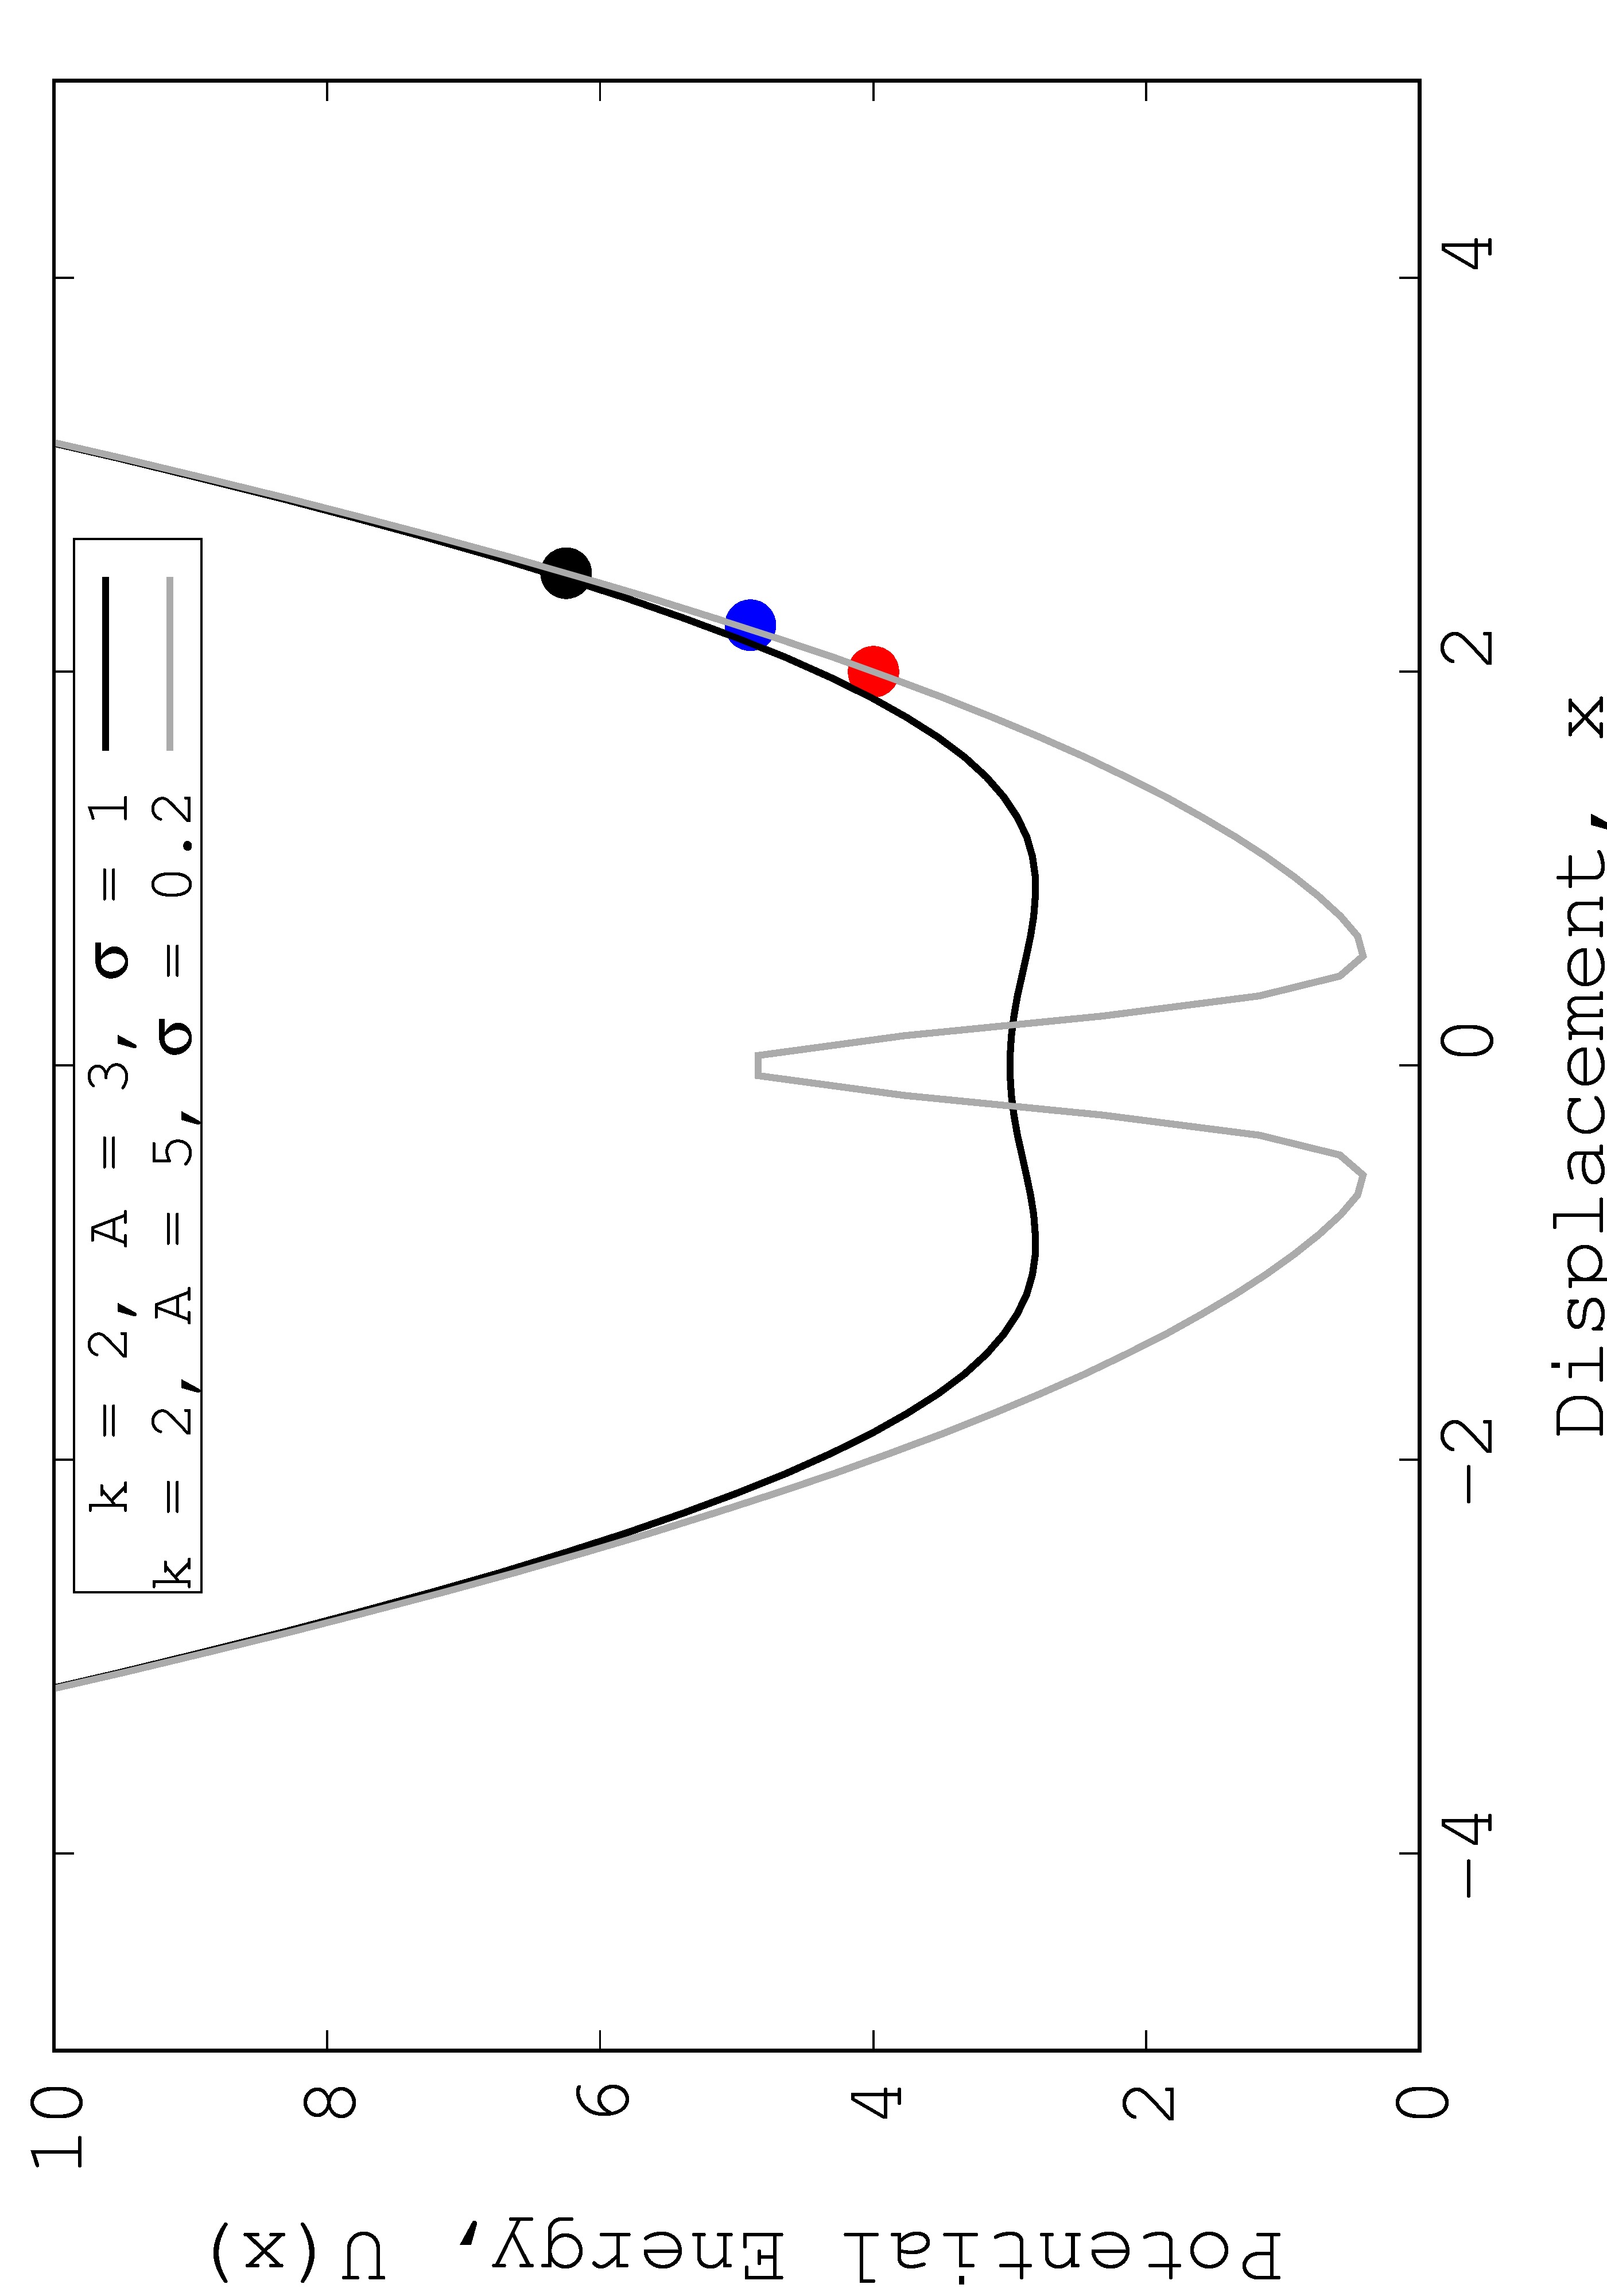
\includegraphics[width=0.7\textwidth,angle=270]{figures/Nov14_plot1.jpg}
\end{figure}
\end{column}
\end{columns}
\end{frame}

\begin{frame}{Conservation of Energy}
\begin{columns}[T]
\begin{column}{0.3\textwidth}
\small
Suppose each particle starts with sufficient negative velocity to cross the origin.  If the velocities were instead positive, which would cross the origin?
\begin{itemize}
\item A: Black only
\item B: Black and Blue
\item C: All
\item D: None
\end{itemize}
\end{column}
\begin{column}{0.7\textwidth}
\begin{figure}
\centering
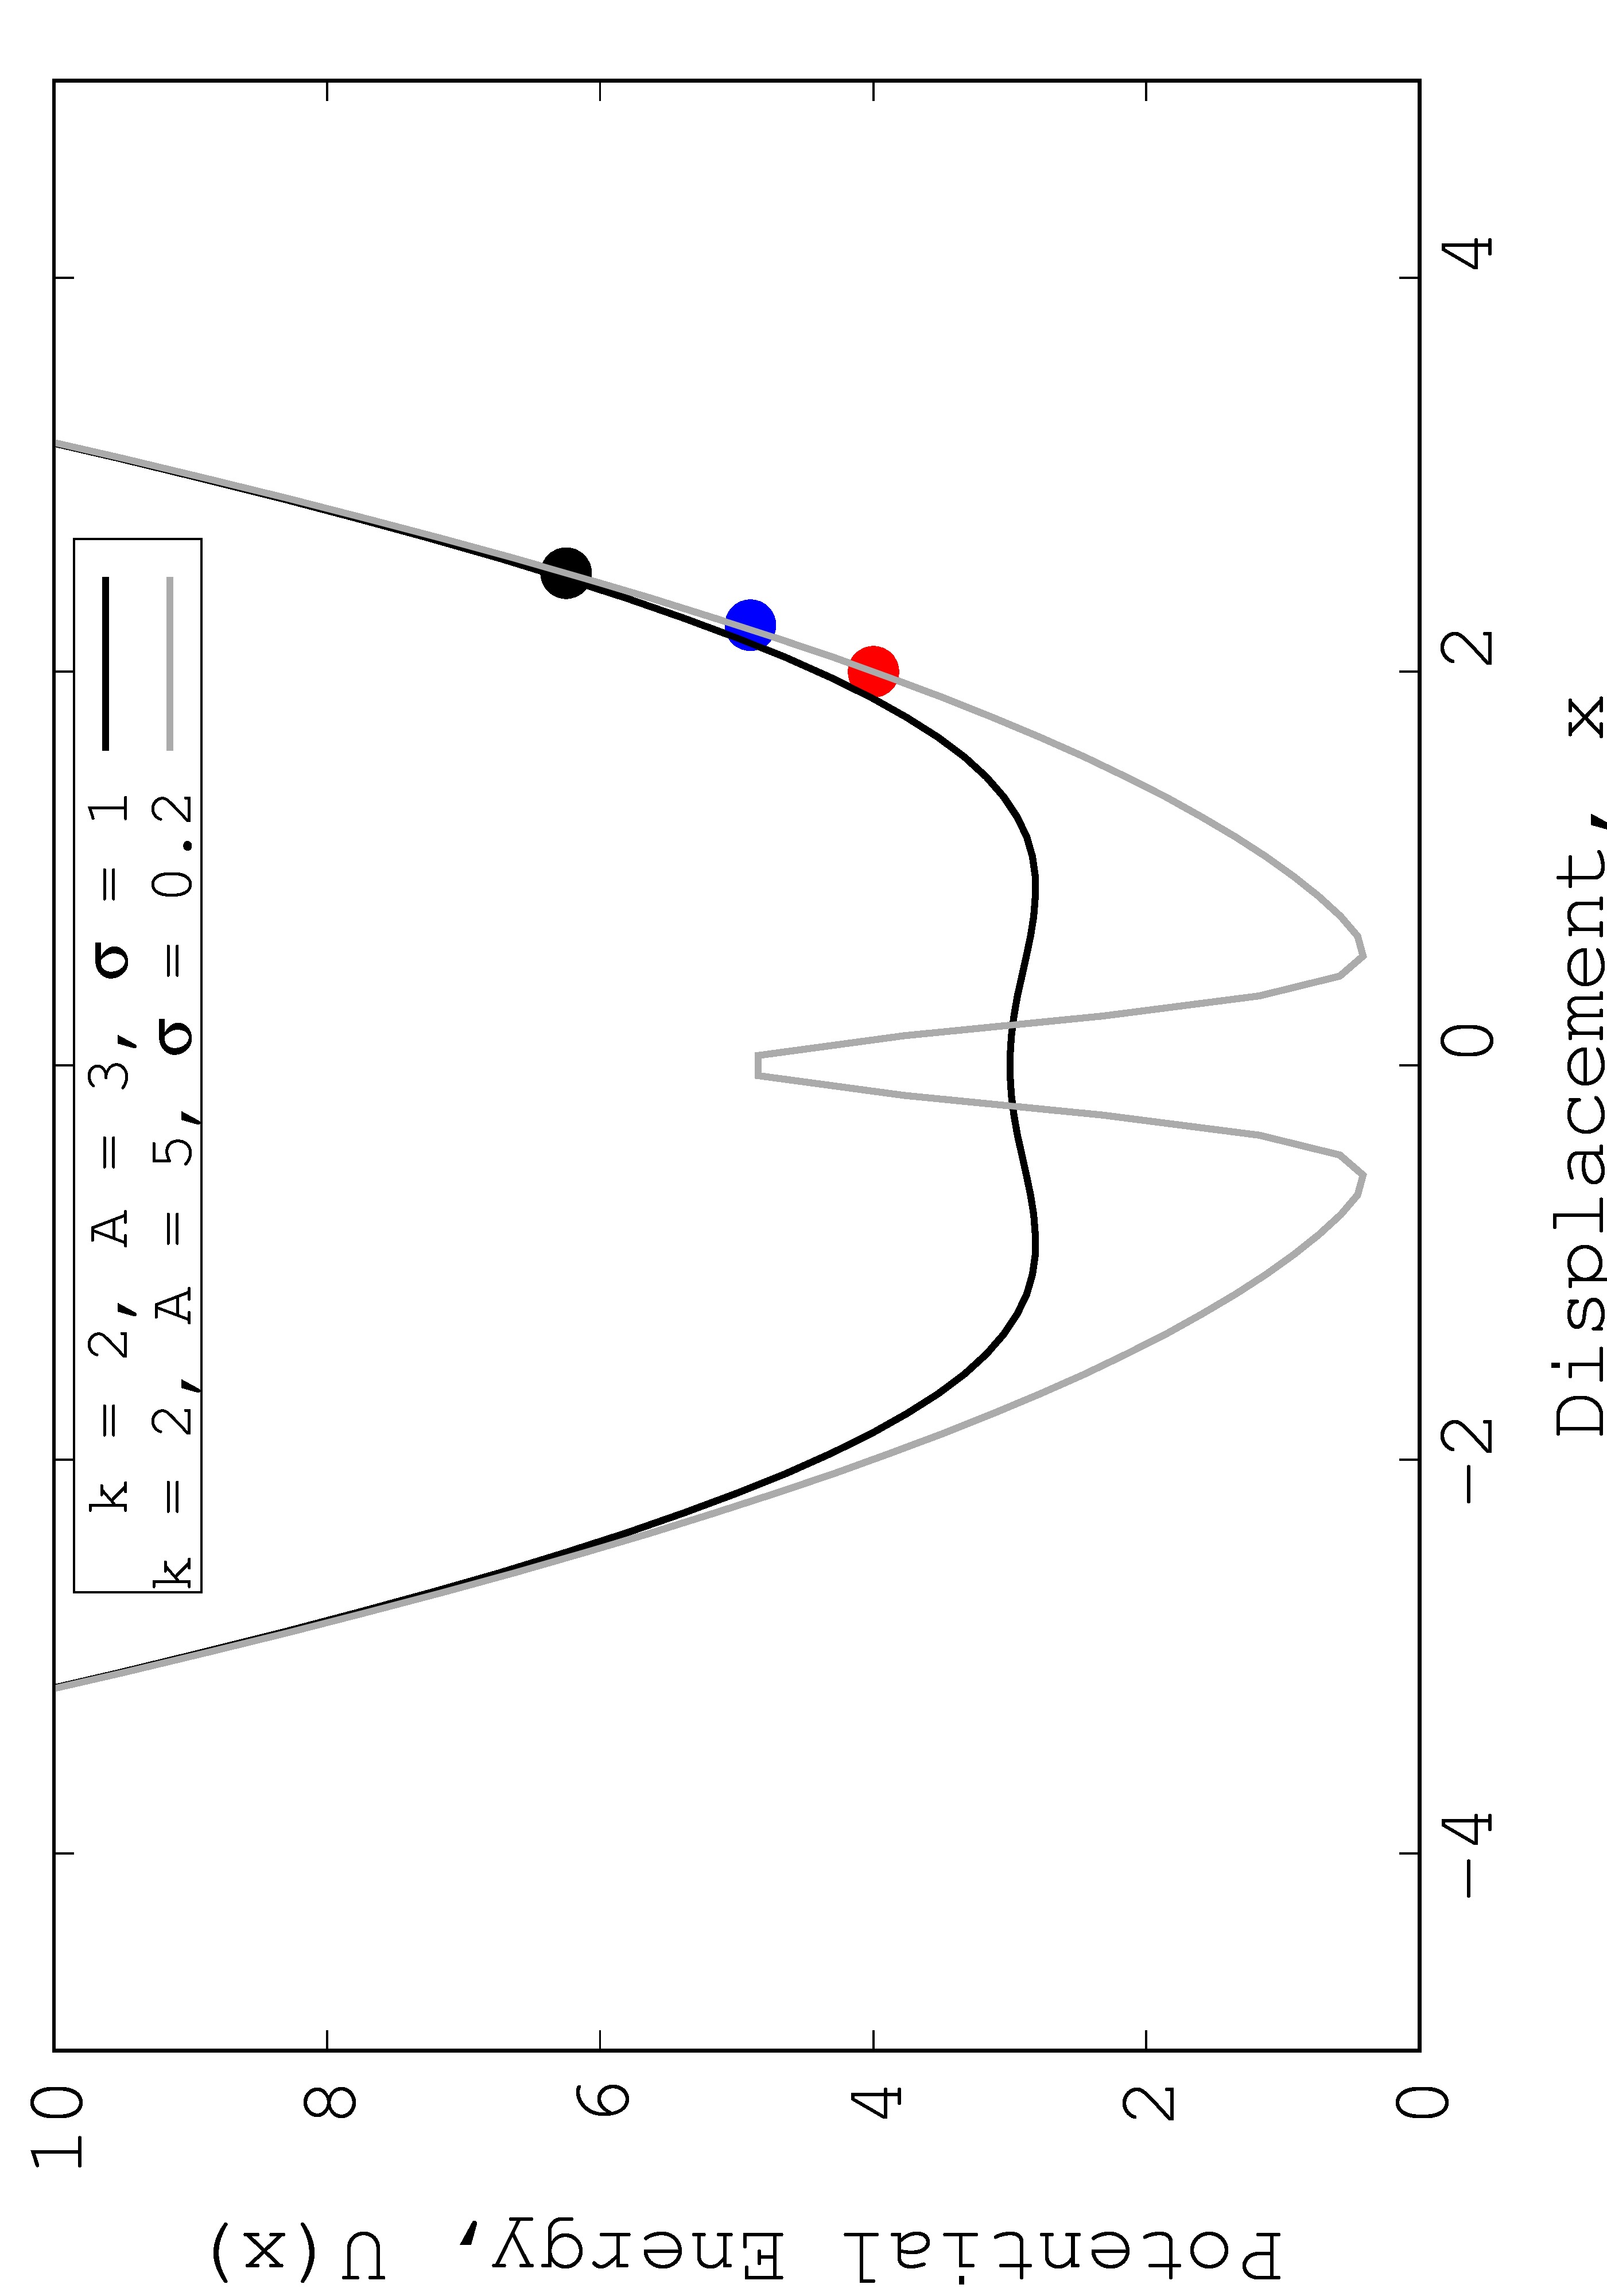
\includegraphics[width=0.7\textwidth,angle=270]{figures/Nov14_plot1.jpg}
\end{figure}
\end{column}
\end{columns}
\end{frame}

\begin{frame}{Conservation of Energy}
\begin{columns}[T]
\begin{column}{0.3\textwidth}
\small
Suppose Black and Red particles begin at $x=0$. Which particle or particles is displaced?
\begin{itemize}
\item A: Black only
\item B: Red and Black
\item C: Red only
\item D: Neither
\end{itemize}
\end{column}
\begin{column}{0.7\textwidth}
\begin{figure}
\centering
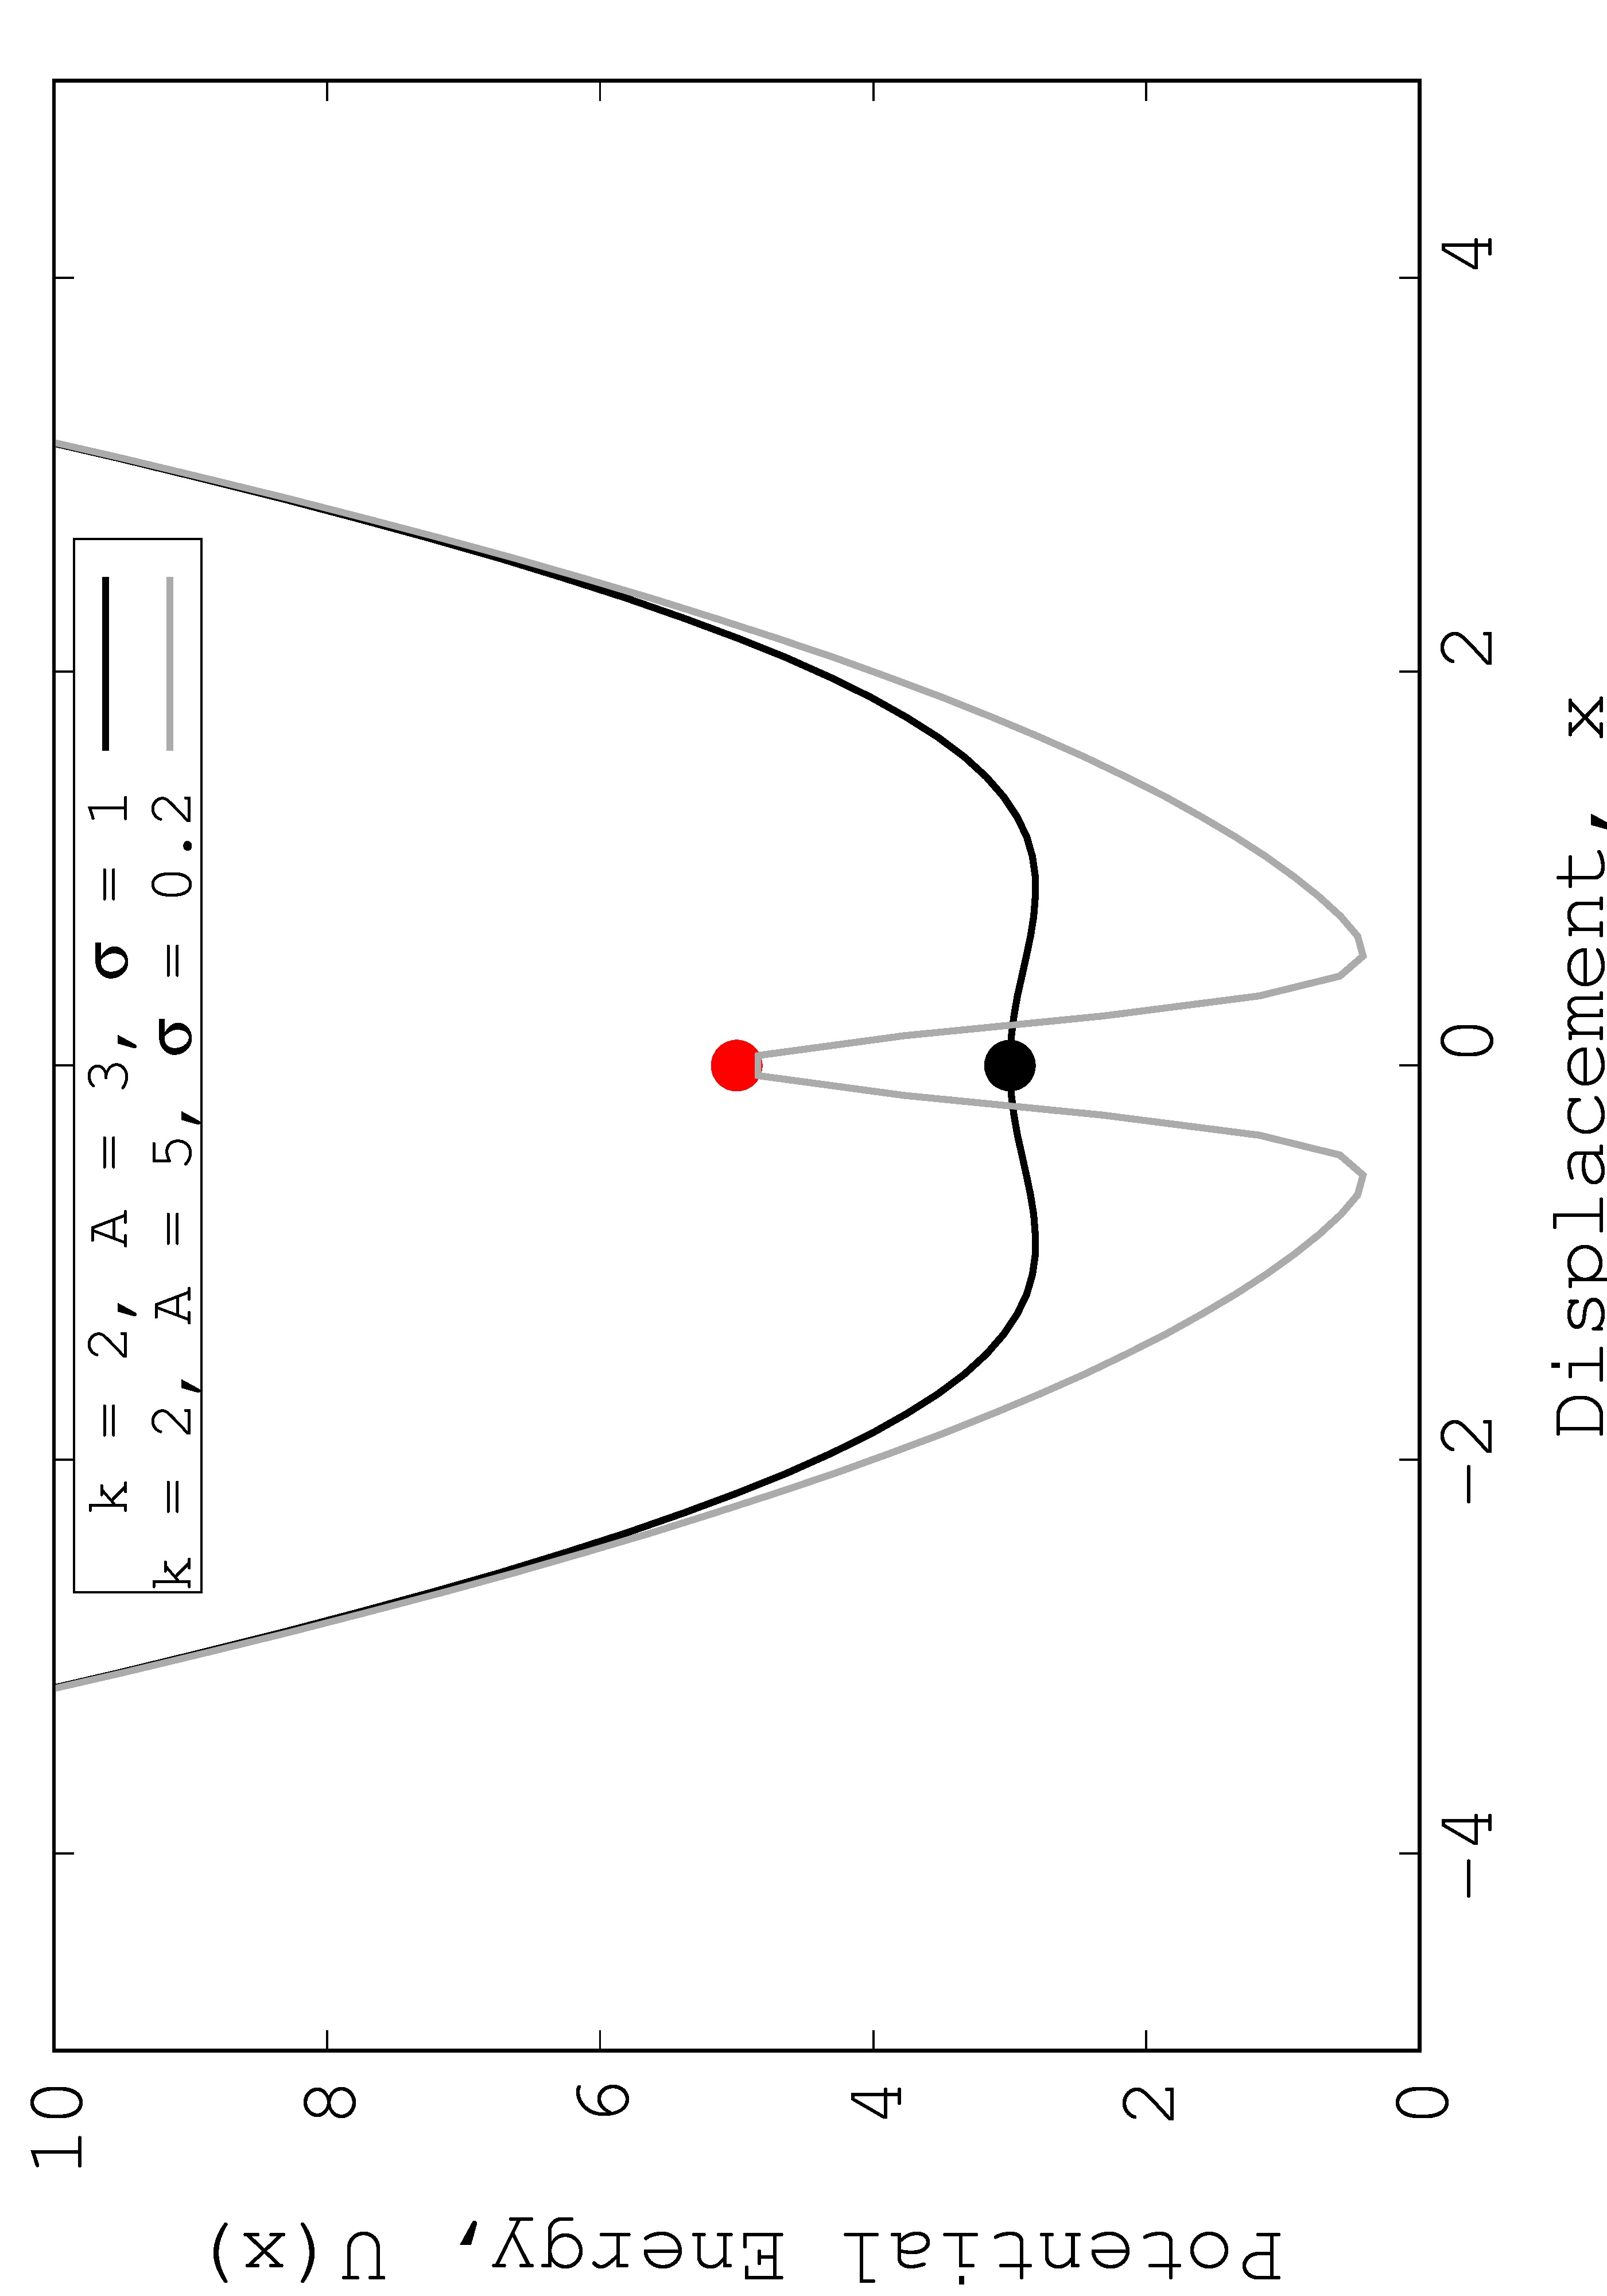
\includegraphics[width=0.7\textwidth,angle=270]{figures/Nov14_plot2.jpg}
\end{figure}
\end{column}
\end{columns}
\end{frame}

\begin{frame}{Conservation of Energy}
\begin{columns}[T]
\begin{column}{0.3\textwidth}
\small
Assuming each particle starts with no velocity, which particle or particles is displaced?
\begin{itemize}
\item A: Black only
\item B: Red and Black
\item C: Red only
\item D: Neither
\end{itemize}
\end{column}
\begin{column}{0.7\textwidth}
\begin{figure}
\centering
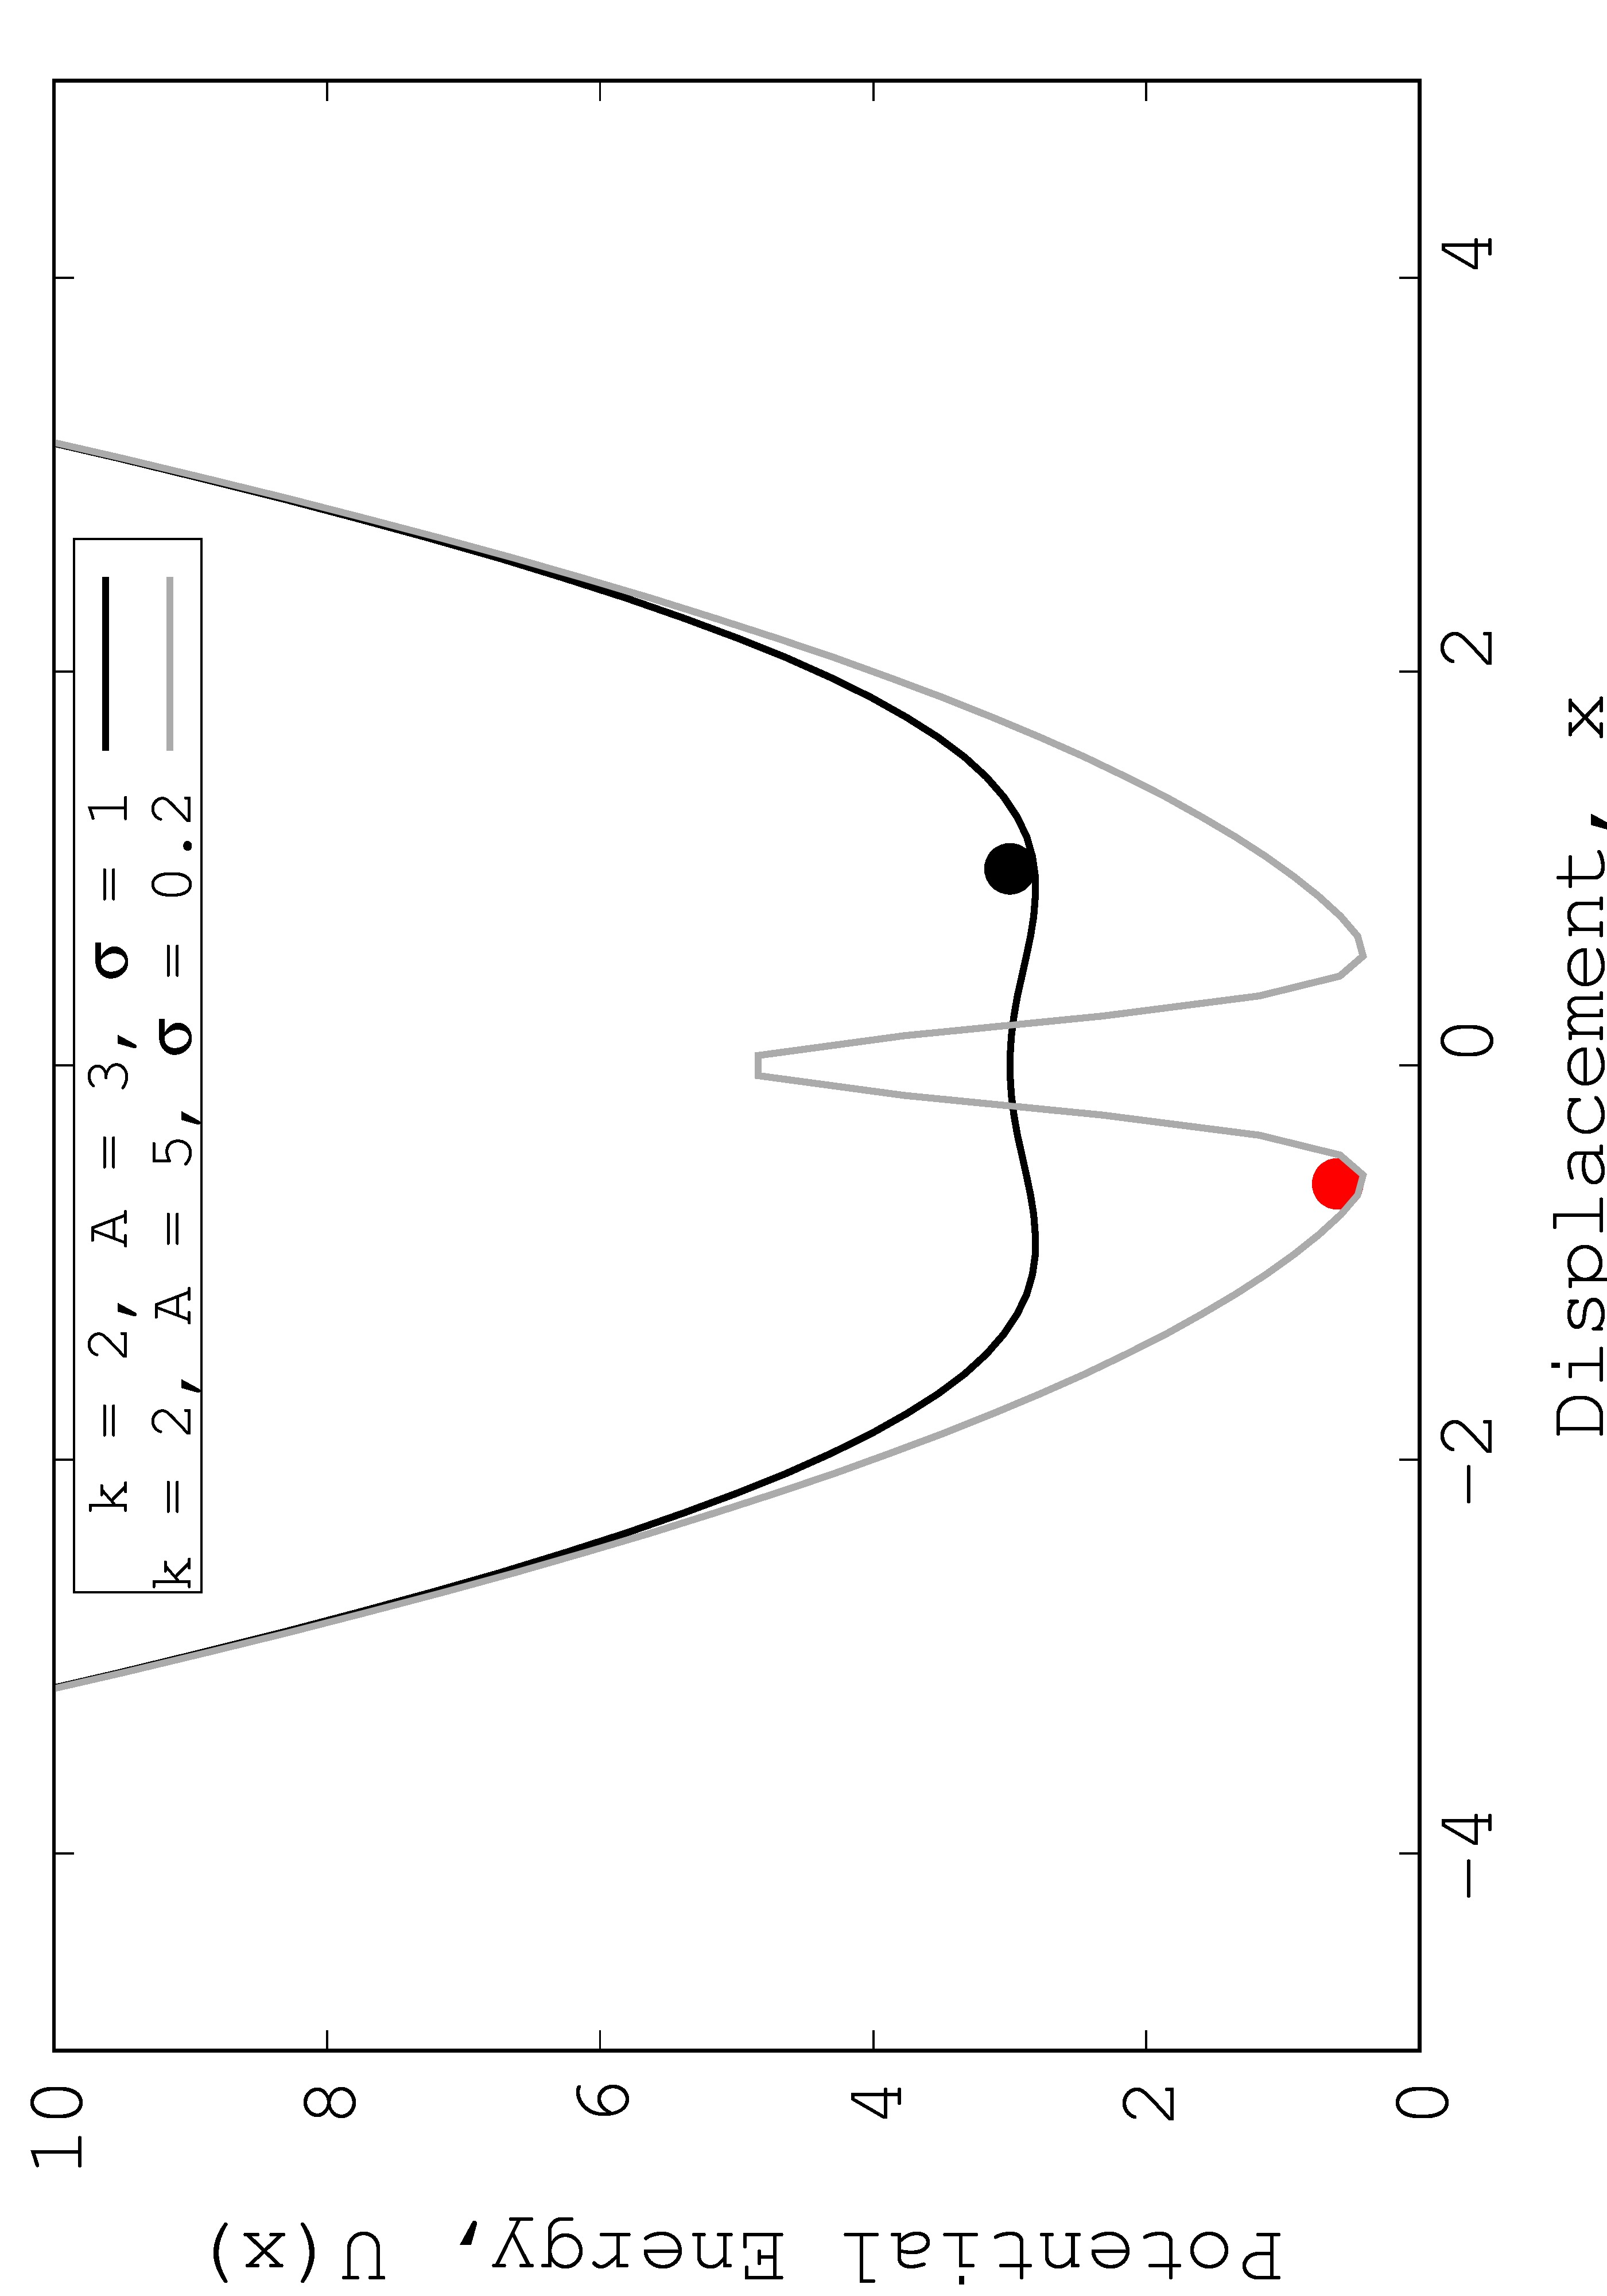
\includegraphics[width=0.7\textwidth,angle=270]{figures/Nov14_plot3.jpg}
\end{figure}
\end{column}
\end{columns}
\end{frame}

\begin{frame}{Conservation of Energy}
\begin{columns}[T]
\begin{column}{0.3\textwidth}
\small
Knowing that $F = -U'$, which of the following is true?
\begin{itemize}
\item A: Red is $F$ of black $U$
\item B: Blue is $F$ of gray $U$
\item C: Red is $F$ of gray $U$
\item D: Blue is $F$ of red $U$
\end{itemize}
\end{column}
\begin{column}{0.7\textwidth}
\begin{figure}
\centering
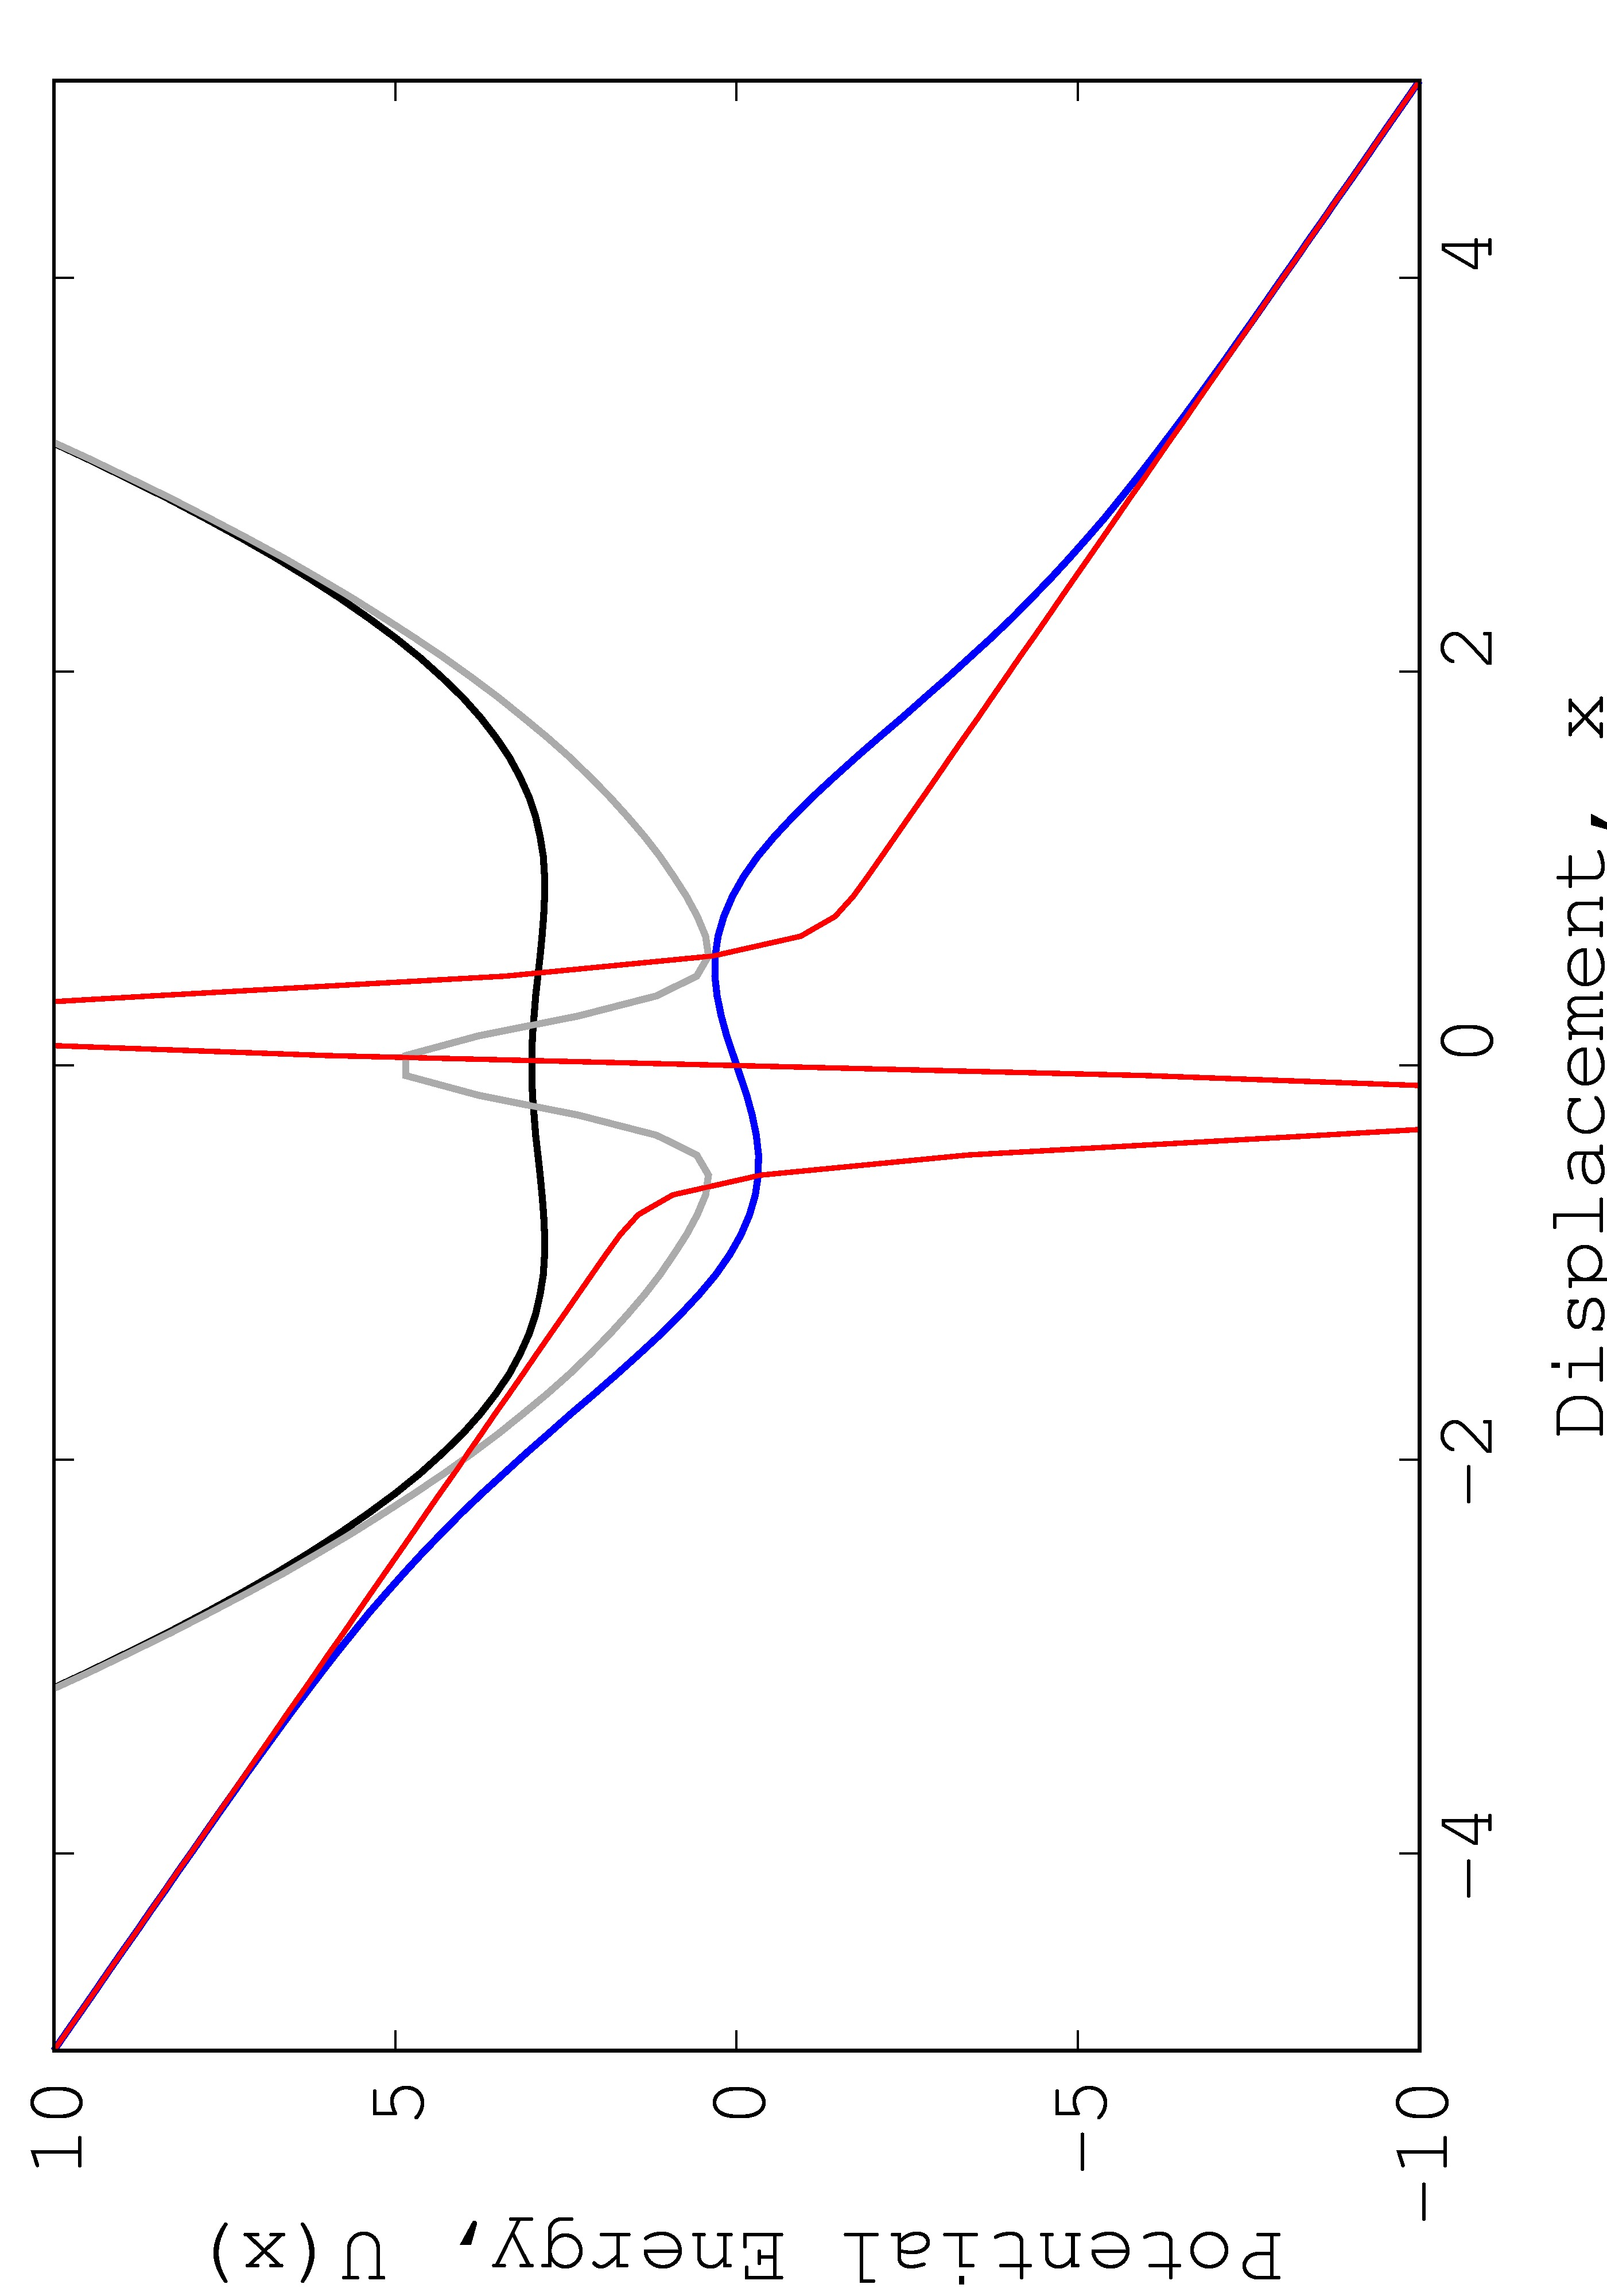
\includegraphics[width=0.7\textwidth,angle=270]{figures/Nov14_plot4.jpg}
\end{figure}
\end{column}
\end{columns}
\end{frame}

\begin{frame}{Conservation of Energy}
\begin{columns}[T]
\begin{column}{0.3\textwidth}
\small
Knowing that $F = -U'$, which of the following is true?
\begin{itemize}
\item A: Blue is $F$ of black $U$
\item B: Red is $F$ of blue $U$
\item C: Red is $F$ of black $U$
\item D: Blue is $F$ of red $U$
\end{itemize}
\end{column}
\begin{column}{0.7\textwidth}
\begin{figure}
\centering
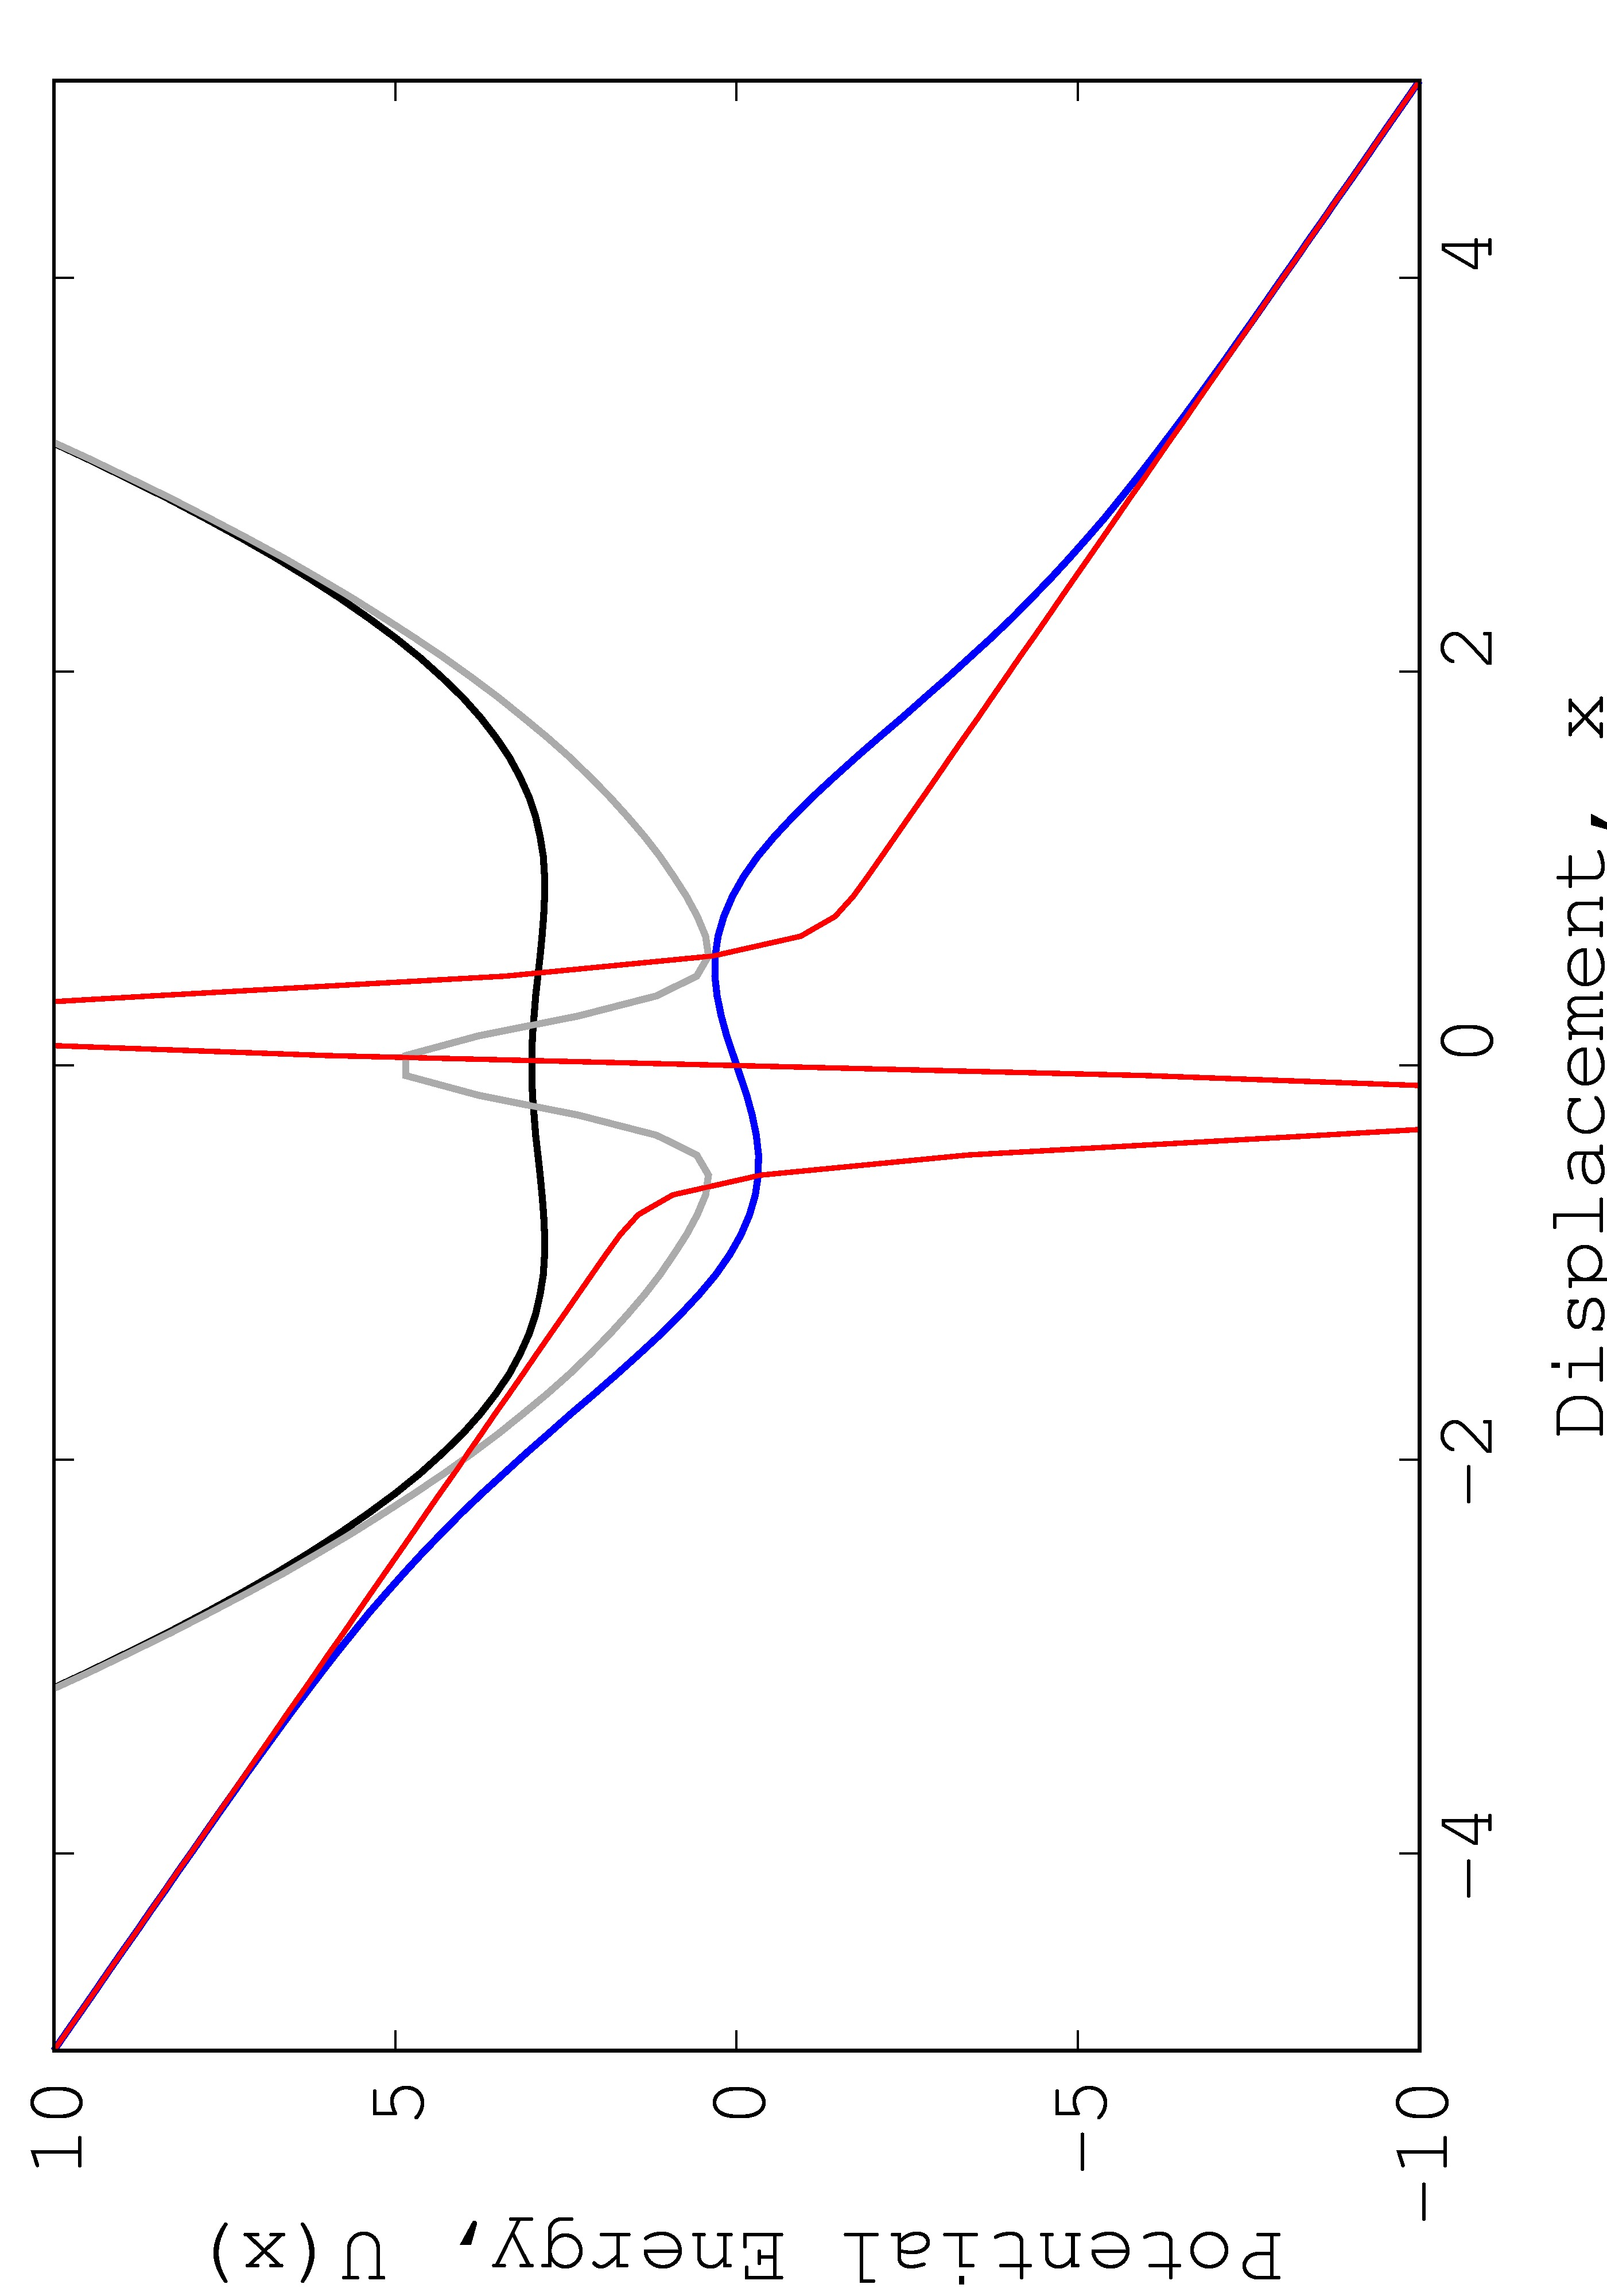
\includegraphics[width=0.7\textwidth,angle=270]{figures/Nov14_plot4.jpg}
\end{figure}
\end{column}
\end{columns}
\end{frame}

\begin{frame}{Conservation of Energy}
\begin{figure}
\centering
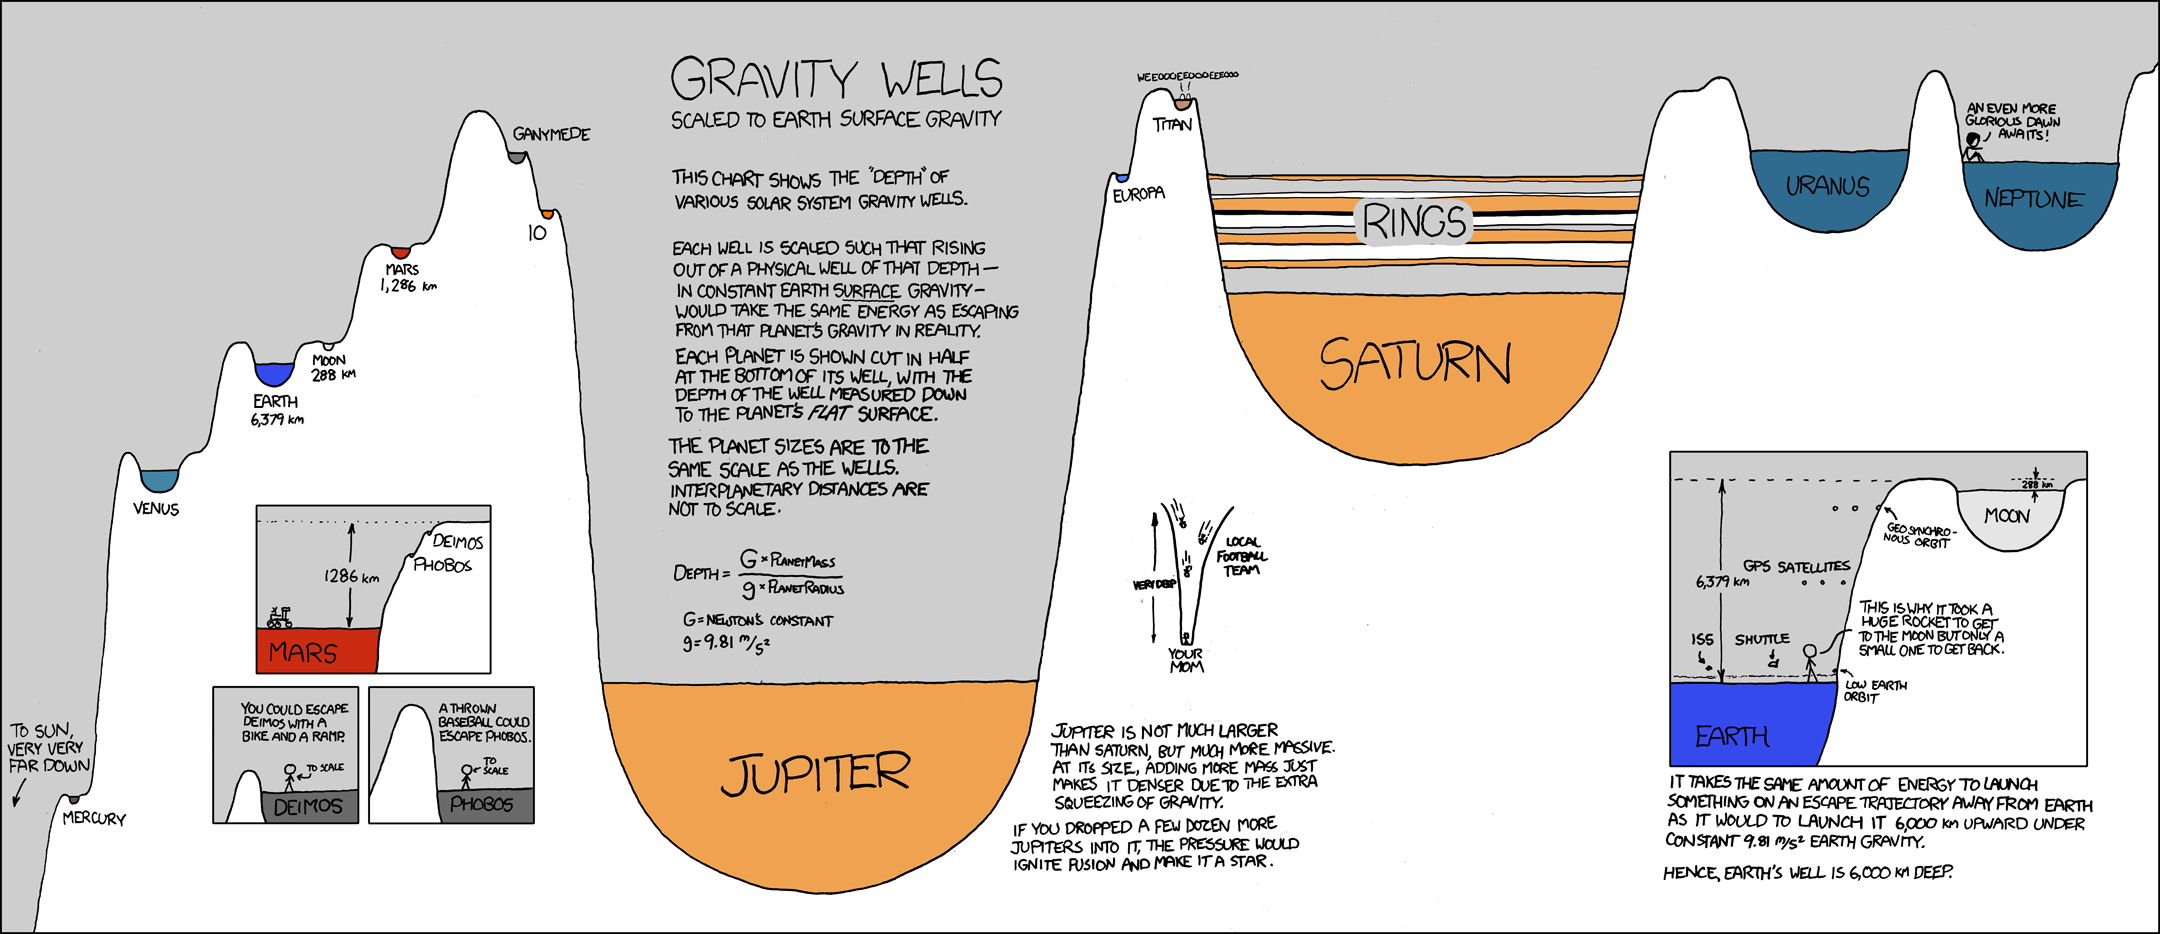
\includegraphics[width=0.95\textwidth]{figures/gravity_wells_large.png}
\caption{\label{fig:well} Potential energy surfaces in the solar system (xkcd.com).}
\end{figure}
\end{frame}

\section{Conclusion}

\begin{frame}{Unit 7 Summary}
\begin{enumerate}
\item \alert{Work} and \alert{potential energy}
\begin{itemize}
\item \textbf{Lab activity:} Oscillator and gravity trading work and potential energy
\end{itemize}
\item Potential energy and \textbf{conservative forces}
\item \alert{\textbf{Conservation of Energy}}
\begin{itemize}
\item \textit{Calculus review: the fundamental theorem of calculus}
\item Graphical representations of integrals and energy
\end{itemize}
\end{enumerate}
\end{frame}

\end{document}
